\subsection{Story: Site should be mobile responsive}
\subsubsection{Analysis - Breakdown of Tasks}
\begin{itemize}
	\item Create standard media query sizes
	\item Create media query for quiz questions
	\item Media query for welcome page
\end{itemize}
\subsubsection{Design}
A quiz page should look like the design specified in iteration 4  (\ref{fig:iter-4-use-case}).
\subsubsection{Implementation}
Finding the media query sizes was simple, Bootstrap recommends some default sizes for phones, tablets etc. (TODO: cite this https://getbootstrap.com/css/\#grid-media-queries ) It was then a simple task of using the Chrome developer tools to view the page in mobile view and change the various sizes of buttons and titles in the CSS editor to be more mobile friendly.
\subsubsection{Testing}
This is not really possible to test with automated testing, but should be easy to test with users later in the project. Additionally once live the system could be tested with the Google Responsive Test site that gives a score for the usability of a site in mobile view.
\newpage

\subsection{Part Two Re-Design}
Originally planned to be an extension to Microsoft PowerPoint or a similar technology, such as Libre Office, this was determined to be a large amount of work (TODO: cite this). This meant an alternative solution had to be devised or some extra requirements had to be added to the system. An alternative solution was found rather than abandon the idea of having slides within the quizzes. Slideshow programs usually have the ability to render their slides as PDF, a format which is more heavily supported compared to a propriety format such as .pptx provided by Microsoft. If a PDF is uploaded to the application, PHP can be used to turn these PDF slides into images, which can then be rendered on the quiz pages.

This new approach means some changes to the original stories for the second part, here are the revised stories for this part:
\begin{itemize}
	\item (1) The admin creates slides in their preferred editor and exports them as a PDF
	\item (4) The admin can upload these slides to a quiz they have created in the past
	\item (3) The admin can reorder the questions within the quiz to move them around the slides
	\item (2) When this quiz is run, it should render the slides as well as questions in the order specified
\end{itemize}

There are some disadvantages to this however. The main issues is that slide animations are not rendered as separate slides on the PDF. There are extensions for Microsoft PowerPoint that let the slides be rendered with animations occupying separate slides so as to provide a "fake" animation. Another problem is that the slides would have to be uploaded before a lecture as it can take a few minutes to render PDF slides as images. This could be argued as an advantage however, if lecturers upload their slides before a lecture they only need to log in to the application when then want to run them, no need to bother carrying the slides on a memory stick or saving them to their University storage.
\newpage

\subsection{Story: The admin can upload these slides to a quiz they have created in the past}
\subsubsection{Analysis - Breakdown of tasks}
\begin{itemize}
	\item Upload pdf slides
	\item Convert these slides to images
	\item Save references to these slides in the database
	\item Show the slides on the Quiz.show page
\end{itemize}
\subsubsection{Design}
See \ref{fig:iter-7-use-case}

\begin{figure}
	\caption{Use case for quiz creation featuring moving questions and the add slides function. See Iteration 2 for more detailed use case diagram of the rest of the backend.}
	\centerline{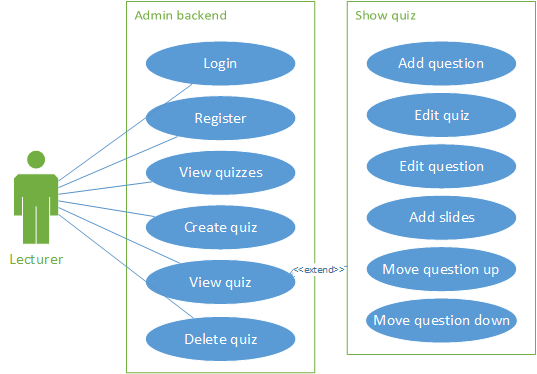
\includegraphics{Chapter2/Iter-7/iter-7-use-case}}
	\label{fig:iter-7-use-case}
\end{figure}

\subsubsection{Implementation}
To upload the slides, it was done with a standard HTML file input but the backend used techniques native to Laravel: (TODO cite: https://laracasts.com/series/whats-new-in-laravel-5-3/episodes/12). These images are then saved in the /storage/app/public/slides folder. Within this, they are organised into folders named after the session id and then quiz id within those.

These slides are then converted using a library that uses Imagick - (TODO: cite this https://github.com/spatie/pdf-to-image). Whilst saving them, references are also saved to the database. This is so that the images can be referenced quickly later on when displaying an slide or question as database reading is quick. For this functionality, a new table for slides was added to the system, storing the file name, quiz it was associated with and a position. 

The last task involved showing the slides and questions on the Quiz.show page. Seeing as the new story involved reordering them, simply rendering the slides after the questions would not do, it should render them in order of the position. The main problem is that there is no simple SQL query that can select two sets of results and then order them by a common column. The easier solution was to create a PHP function to create an array of all the items in the order wanted. (TODO: Cite this function in appendix, should I explain here or in the appendix?)
\subsubsection{Testing}
\newpage

\subsection{Story: The admin can reorder the questions within the quiz to move them around the slides}
\subsubsection{Analysis - Breakdown of tasks}
\begin{itemize}
	\item Add buttons to reorder questions
	\item This button increases or decreases position of question
	\item It swaps the positions of two questions or a slide and question if required
	\item Add some limits to positioning like not going below 1
\end{itemize}
\subsubsection{Design}
As a minor change to the system, no major design choices were made here. Simple Bootstrap icons can be used for the position changing arrows, which is the only front end change.
See \ref{fig:iter-7-use-case} 
\subsubsection{Implementation}
Main functionality to add was the changing of positions. This was rather simple, adding a simple Route and buttons that triggered the actions associated with the new route. It was decided that the Route would be a POST request rather than GET as technically it is submitting some data, the direction and id of the question. The action it calls simply updates the position in the database after doing some checks of the position it wants to move to. If it is already occupied, it swaps the object at the new position with its current position. This object could be a question or slide.   
\subsubsection{Testing}
\newpage

\subsection{Story: When the quiz is run, it should render the slides as well as question in the order specified}
\subsubsection{Analysis - Breakdown of tasks}
\begin{itemize}
	\item Find the position in the database and decide whether its a slide or question
	\item Render a question like normal
	\item If a slide, render a simple img tag and populate with the image name from the WebSockets
	\item Resize image to fit the page, including for mobile responsive
	\item Render question by default for users joining late
\end{itemize}
\subsubsection{Design}
This should work in much the same way as the questions, in that it will send an Ajax request to a page with the image name and then copy the content of the ajax page into the live page. The content page to Ajax should be pretty simple, a simple container with an img tag. The other tasks are extensions to previously created functions.
\subsubsection{Implementation}
The first task is to determine what is at the position, this involved changing the current function to check if the question at the requested position was null, if it was then it should find a slide at the specified position. As well as the data about the slide or question, it would return a type so that when it was called the system knew what type of content it was to expect. The data was then sent to the WebSockets and another case was added to the JavaScript receiving end for triggering an AJAX call to a slide page. This page would render a simple img tag with the slide specified which is then added to the current page like the questions.

A problem with rendering the images was the files stored within the /storage folder are not publicly accessible, usually only files within the /public folder are. However, there is a simple artisan command to create a symlink from the public folder that points to the storage/app/public folder. TODO add command: php artisan storage:link
\subsubsection{Testing}
\newpage